\subsection{预备结果}

引理 1. 超平面集 \(\mathfrak{H}\) 是局部有限的。

事实上，设 K 是 E 的一个紧子集。若超平面 \(H \in H\) 与 K 相交，则集合 \(s_{\mathrm{H}}(\mathrm{K})\) 也与 K 相交，因为 \(K \cap H\) 中的每个点都被 \(s_{H}\) 固定。因此，与 K 相交的 \(H \in H\) 的集合由 (D'2) 可知是有限的。

因此，我们可以将 §1 的定义和结果应用于 E 和 H。我们将 E 中由 H 定义的室、面片、墙等统称为相对于 W 的室、面片、墙等。任意位移 \(w \in W\) 都置换室、面片、墙等。

引理 2. 设 C 是一个室。

\begin{enumerate}
\def\labelenumi{(\roman{enumi})}
\item
对于任意 \(x \in \mathrm{E}\)，存在 \(w \in \mathrm{W}\)，使得 \(w(x) \in \overline{\mathrm{C}}\)。
\item
对于任意室 \(\mathrm{C}'\)，存在 \(w \in \mathrm{W}\)，使得 \(w(\mathrm{C}') = \mathrm{C}\)。
\item
群 W 由关于 C 的墙的正交反射所成的集合生成。
\end{enumerate}

令 M 为 C 的墙的集合，令 \(W_{M}\) 为 W 中由关于 C 的墙的反射生成的子群。

\begin{enumerate}
\def\labelenumi{(\roman{enumi})}
\tightlist
\item
设 \(x \in E\)，令 \(J\) 为 \(x\) 在群 \(W_{\mathfrak{M}}\) 作用下所得的轨道。只需证明 \(J\) 与 \(\overline{C}\) 相交。
\end{enumerate}

令 \(a\) 为 \(C\) 的一个点；存在一个闭球 \(B\)，其中心为 \(a\)，且与 \(J\) 相交；由于 \(B\) 是紧的，编号 1 的 (D'2) 性质表明 \(B \cap J\) 是有限集。因此，存在 \(y\) 是 \(J\) 中的一点，使得

\[
d (a, y) \leqslant d (a, y ^ {\prime}) \quad \text { for   all } y ^ {\prime} \text { in } J.\tag{1}
\]

由此，我们将证明 \(y \in \overline{\mathbb{C}}\)。为此，只需证明：若 \(H\) 是 \(C\) 的墙，则 \(y \in \overline{\mathrm{D}_{\mathrm{H}}(C)}\)（参见《一般拓扑》第 §1 第 4 号命题 9）。由于 \(s_H \in W_{\mathfrak{M}}\)，有 \(s_H(y) \in J\)，因而（见图 1）

\[
d (a, y) ^ {2} \leqslant d (a, s _ {\mathrm{H}} (y)) ^ {2}\tag{2}
\]

存在 \(b \in \mathbf{H}\) 以及两个向量 \(t\) 和 \(u\)，使得 \(a = b + t\) 且 \(y = b + u\)，其中向量 \(u\) 与 \(\mathbf{H}\) 正交；于是 \(s_{\mathrm{H}}(y) = b - u\)，而 (2)

等价于 \((t - u|t - u) \leqslant (t + u|t + u)\)，或等价于 \((t|u) \geqslant 0\)。此不等式推出 \(y \in \overline{\mathrm{D}_{\mathrm{H}}(\mathrm{C})}\)。

\pandocbounded{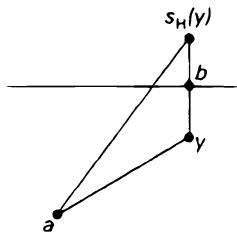
\includegraphics[keepaspectratio]{images/part001_5f5a2798.jpg}}\\
图 1

\begin{enumerate}
\def\labelenumi{(\roman{enumi})}
\setcounter{enumi}{1}
\item
设 \(\mathbf{C}'\) 是一个室且 \(a' \in \mathbf{C}'\)。由已证结果，存在 \(w \in \mathrm{W}_{\mathfrak{M}}\)，使得 \(w^{-1}(a') \in \overline{\mathbf{C}}\)；因此，室 \(\mathbf{C}'\) 与 \(\overline{w(\mathbf{C})}\) 相交；由于 \(\overline{w(\mathbf{C})}\) 是 \(w(\mathbf{C})\) 与内部为空的面片的并（《一般拓扑》第 §1 第 2 号命题 3），故 \(\mathbf{C}' = w(\mathbf{C})\)。
\item
我们必须证明 \(W = W_{\mathfrak{M}}\)，为此只需证明 \(s_{H'} \in W_{\mathfrak{M}}\) 对所有 \(H' \in \mathfrak{H}\) 成立。现在，\(H'\) 至少是一个室 \(C'\) 的墙（《一般拓扑》第 §1 第 4 号命题 8）；我们已经看到，存在 \(w \in W_{\mathfrak{M}}\) 使 \(C' = w(C)\)；于是存在一个墙 \(H\) 属于 \(C\)，使 \(H' = w(H)\)，从而 \(s_{H'} = w.s_H.w^{-1} \in W_{\mathfrak{M}}\)。
\end{enumerate}

